\begin{blocksection}

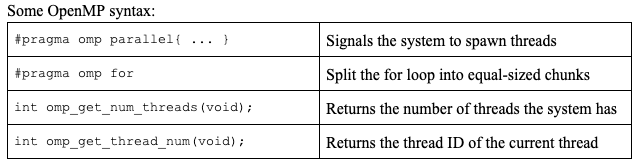
\includegraphics[width=\textwidth]{parallelism/openmp}

\question
Implement the following function using openMP:
\begin{verbatim}
// Sequential code
static int selective_product_total (int n, int *a, int c) {
    for (int i = 0; i < n; i += 1) {
        a[i] = (a[i] > c)? 10 : 0;
}
\end{verbatim}

\begin{parts}
\part
Given the number of elements in a is a multiple of 16, manually distribute the iterations such that there are four contiguous chunks and no false sharing. 
Assume the total number of threads is a multiple of 4. \\
int omp\_get\_num\_threads $\leftarrow$ returns total number of threads in a team \\
int omp\_get\_thread\_num $\leftarrow$ returns current thread ID number

\begin{verbatim}
// openMP code
static int selective_product_parallelized (int n, int *a, int c) {
    #pragma omp parallel {
    for (int i = 0; i < n; i += 1) {
        if ( _____________________________________________) {
                    a[i] = (a[i] > c)? 10 : 0;
                }
            }
    }
}
\end{verbatim}

\begin{solution}[0.5in]
\begin{verbatim}
if (( i / (n/omp_get_num_threads()) ) == omp_get_thread_num()) {
\end{verbatim}
\end{solution}
\end{parts}
    
\end{blocksection}